\documentclass[12pt]{amsart}
\usepackage{geometry}                % See geometry.pdf to learn the layout options. There are lots.
\geometry{letterpaper}                   % ... or a4paper or a5paper or ... 
%\geometry{landscape}                % Activate for for rotated page geometry
%\usepackage[parfill]{parskip}    % Activate to begin paragraphs with an empty line rather than an indent
\usepackage{graphicx}
\usepackage{amssymb}
\usepackage{epstopdf}
\DeclareGraphicsRule{.tif}{png}{.png}{`convert #1 `dirname #1`/`basename #1 .tif`.png}

\usepackage{epsf}
\usepackage{geometry}
\geometry{letterpaper}                   % ... or a4paper or a5paper or ...
\usepackage{listings} 
\usepackage{algorithmic,algorithm}
\usepackage[notcite,notref]{showkeys}
\usepackage{multirow}
\usepackage{enumerate}


\usepackage{amsmath, amsfonts, amssymb,mathrsfs}
%\usepackage{subfigure,pstricks,pst-node}
%\usepackage{pst-eps,epstopdf}
\usepackage{verbatim}
%\usepackage{showkeys}

\everymath{\displaystyle}
\newtheorem{theorem}{Theorem}
\newtheorem{lemma}[theorem]{Lemma}
\newtheorem{corollary}[theorem]{Corollary}

\theoremstyle{remark}
\newtheorem{remark}{Remark}[section]

\theoremstyle{definition}
\newtheorem{definition}{Definition}[section]
\newtheorem{assumption}{Assumption}[section]

\numberwithin{equation}{section} \numberwithin{table}{section}
\numberwithin{figure}{section}
\numberwithin{algorithm}{section}
\numberwithin{theorem}{section}


%\title{}
%\author{The Author}
%\date{}                                           % Activate to display a given date or no date

\begin{document}


\begin{figure}[h!]
	\centering
	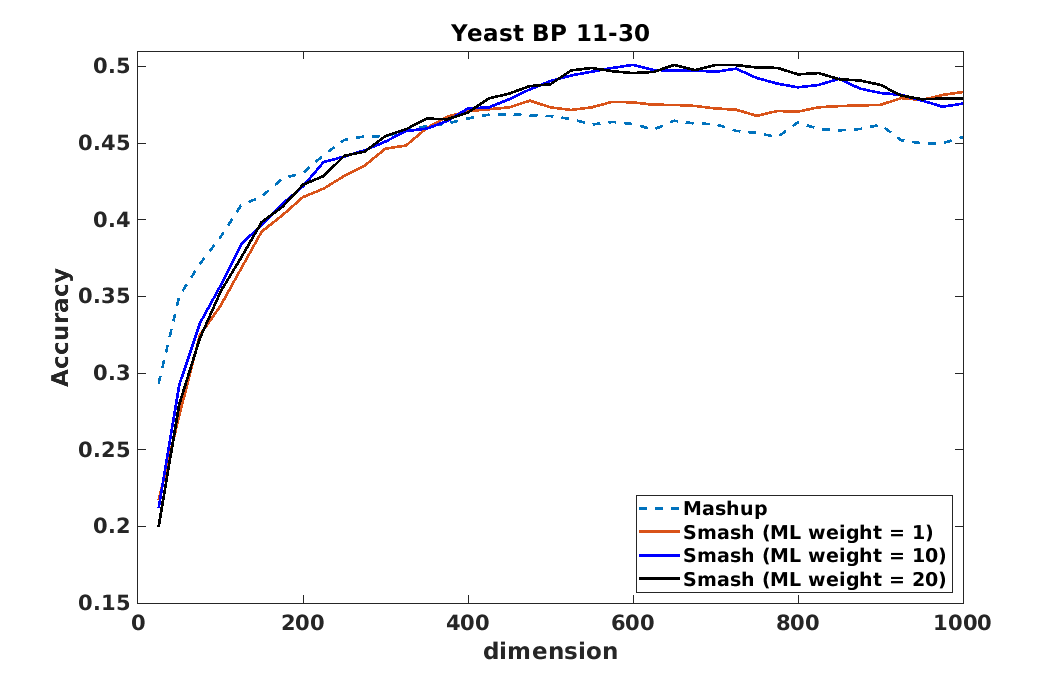
\includegraphics[width=.8\linewidth]{Yeast-BP-11-30-Acc}  \\
	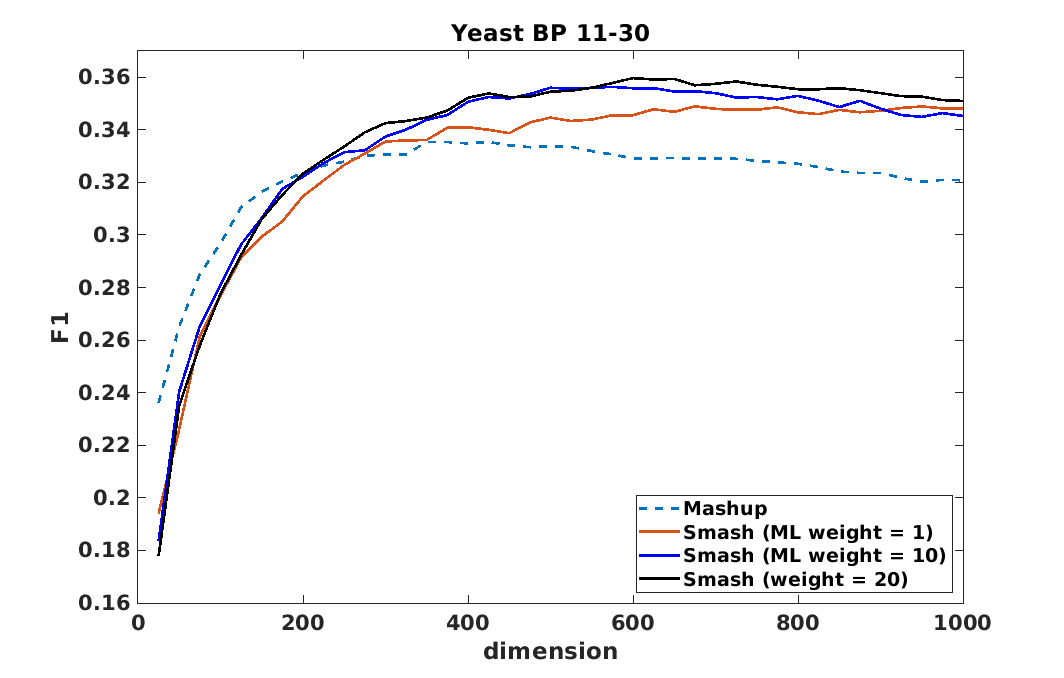
\includegraphics[width=.8\linewidth]{Yeast-BP-11-30-F1}  \\
	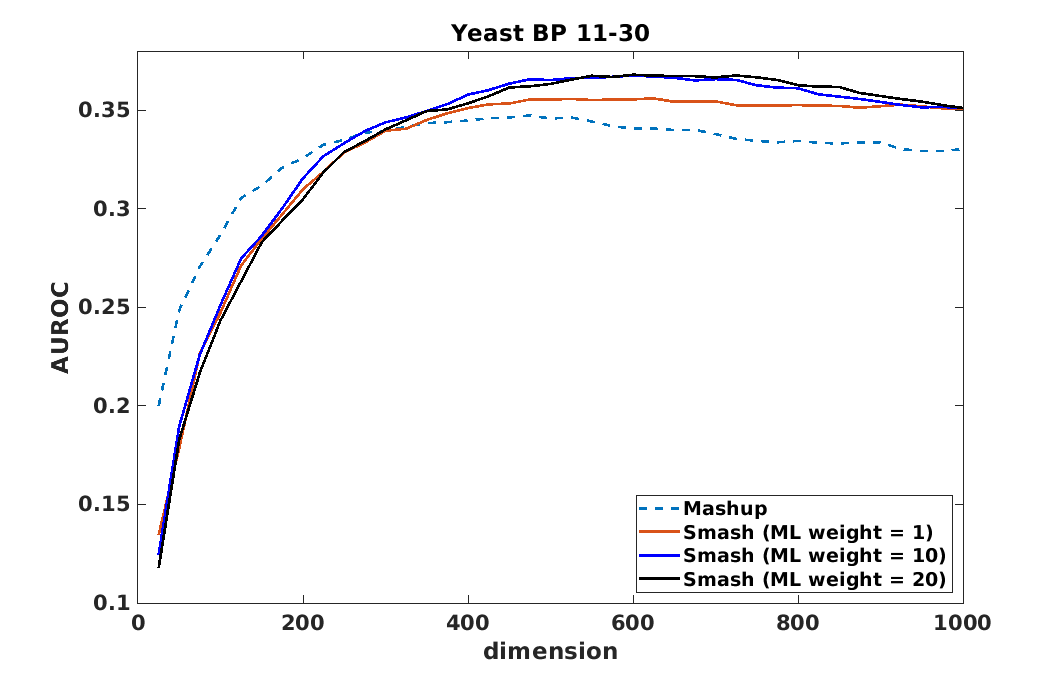
\includegraphics[width=.8\linewidth]{Yeast-BP-11-30-AUROC} 
	%\caption{Yeast BP}
	%\label{fig:yeast-bp}
\end{figure}

\begin{figure}[h!]
	\centering
	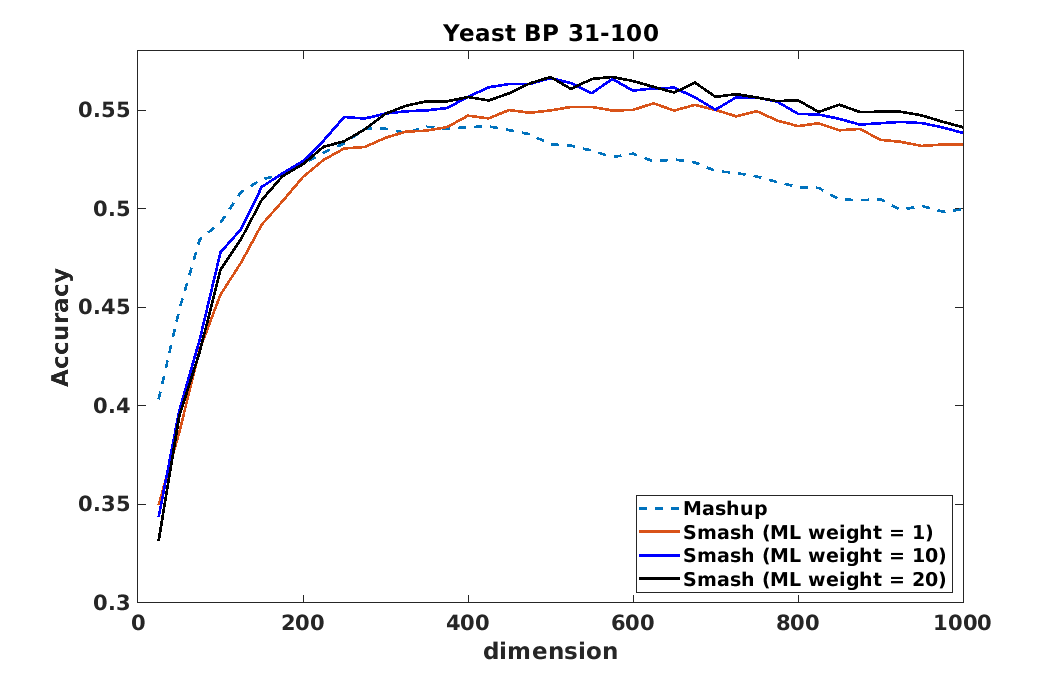
\includegraphics[width=.8\linewidth]{Yeast-BP-31-100-Acc}  \\
	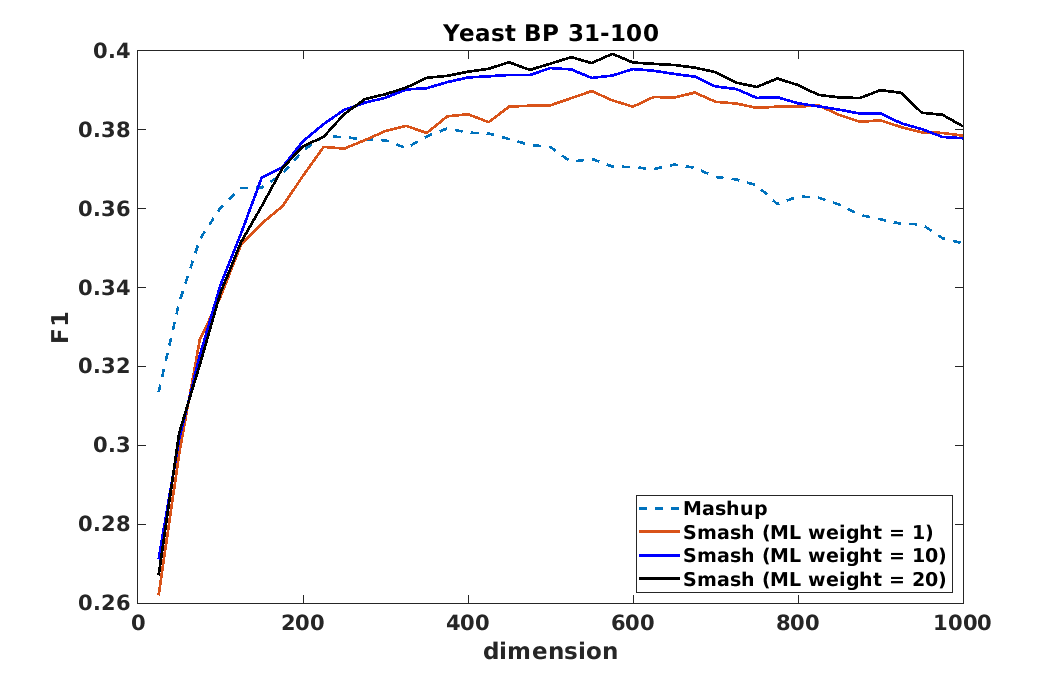
\includegraphics[width=.8\linewidth]{Yeast-BP-31-100-F1}  \\
	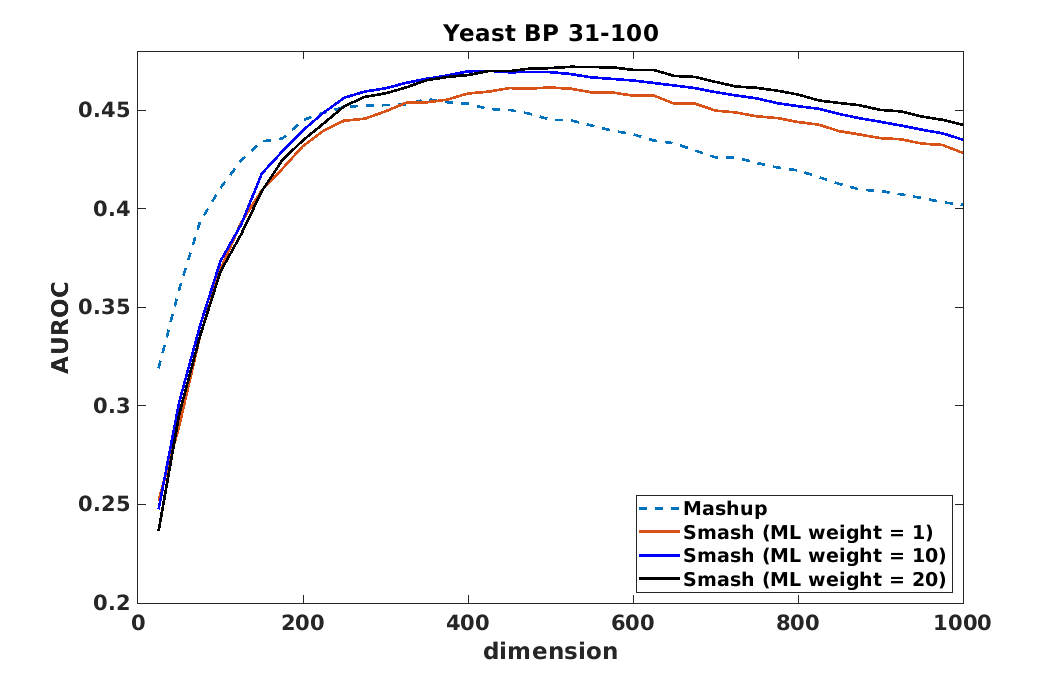
\includegraphics[width=.8\linewidth]{Yeast-BP-31-100-AUROC} 
	%\caption{Yeast BP}
	%\label{fig:yeast-bp}
\end{figure}

\begin{figure}[h!]
	\centering
	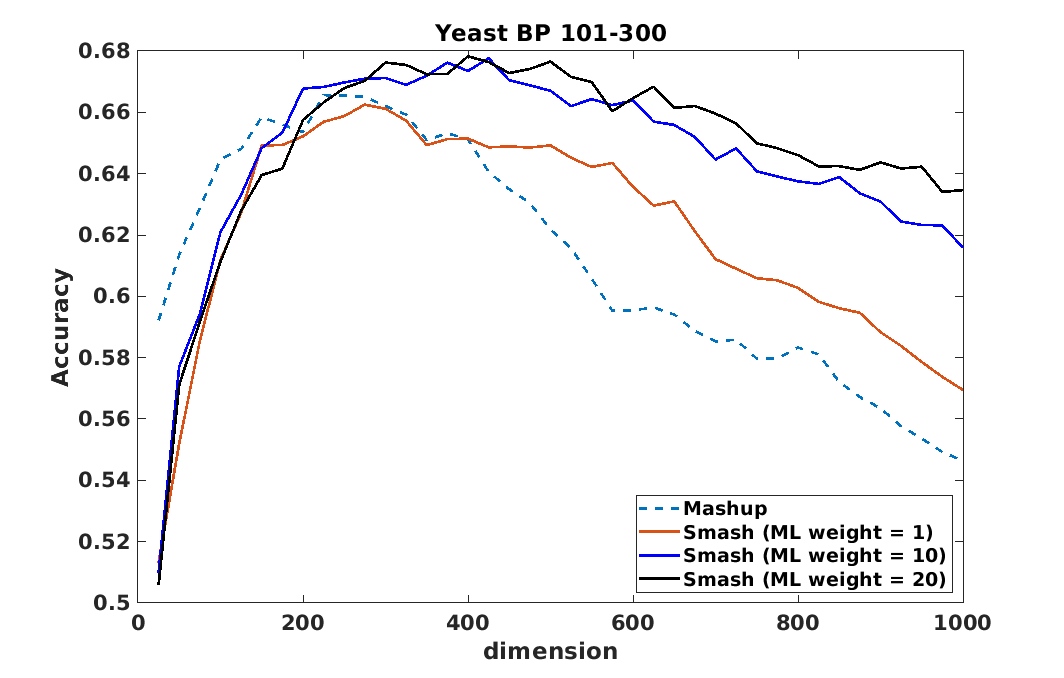
\includegraphics[width=.8\linewidth]{Yeast-BP-101-300-Acc}  \\
	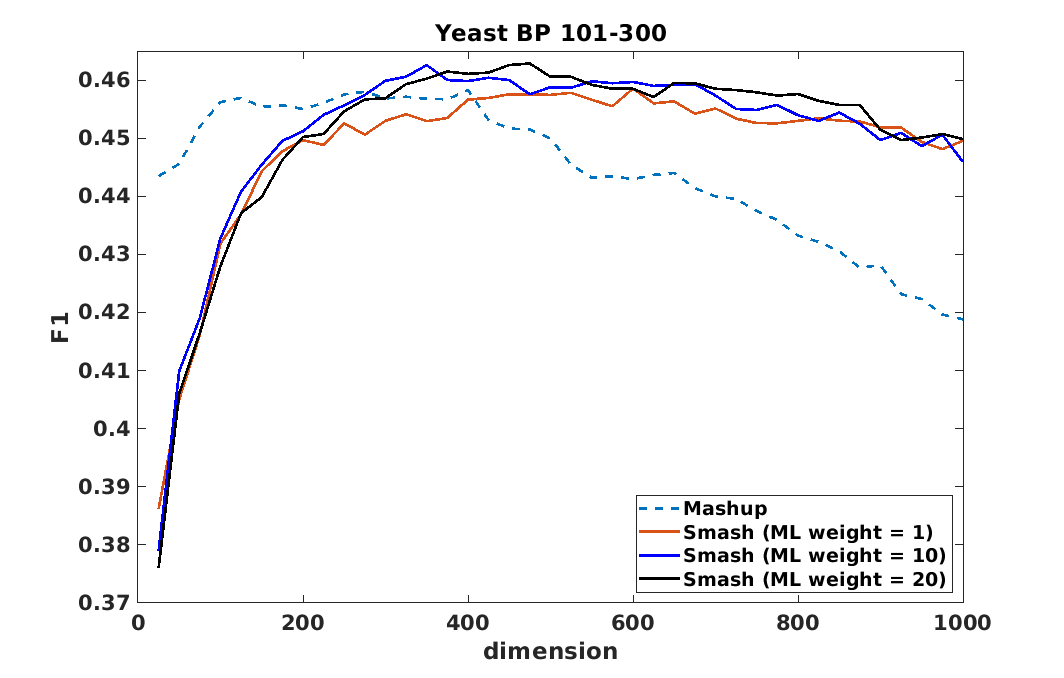
\includegraphics[width=.8\linewidth]{Yeast-BP-101-300-F1}  \\
	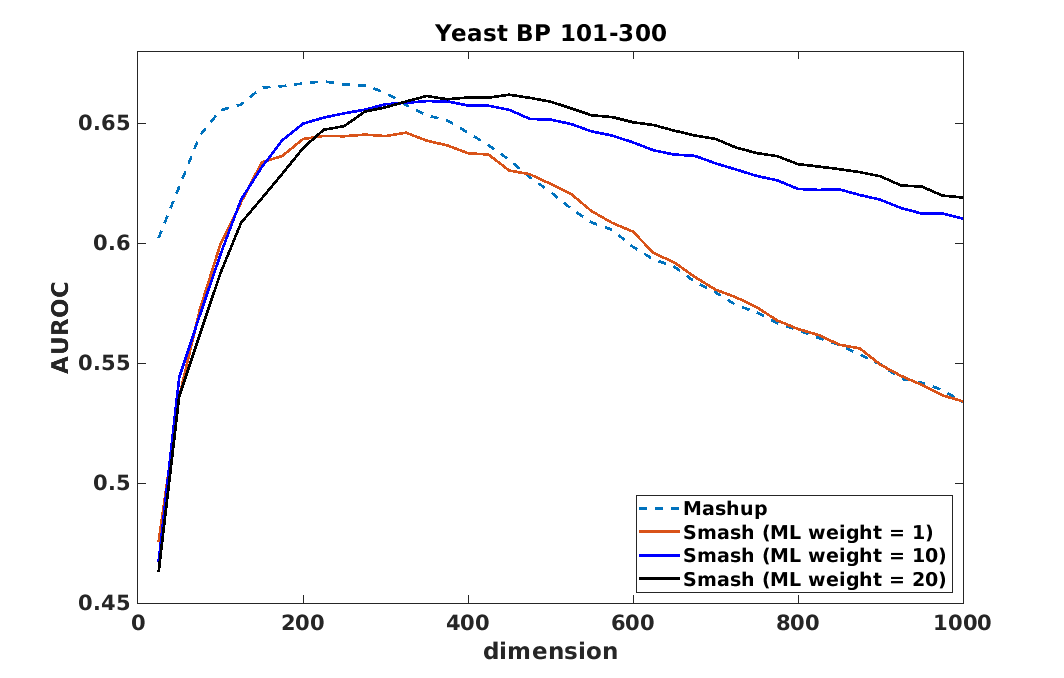
\includegraphics[width=.8\linewidth]{Yeast-BP-101-300-AUROC} 
	%\caption{Yeast BP}
	%\label{fig:yeast-bp}
\end{figure}

\begin{figure}[h!]
	\centering
	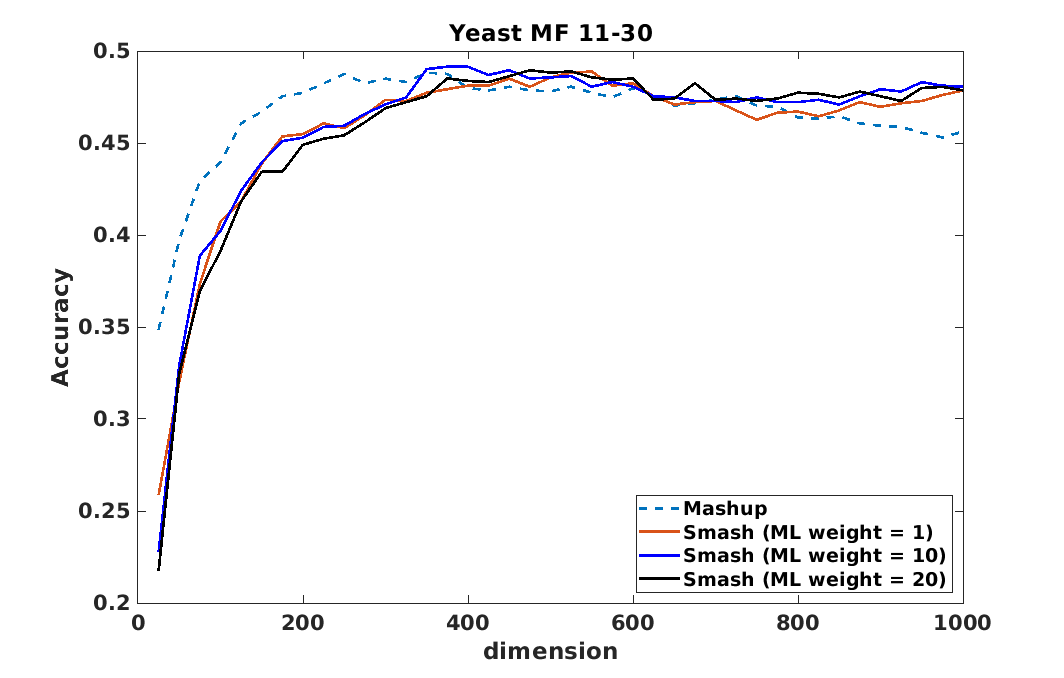
\includegraphics[width=.8\linewidth]{Yeast-MF-11-30-Acc}  \\
	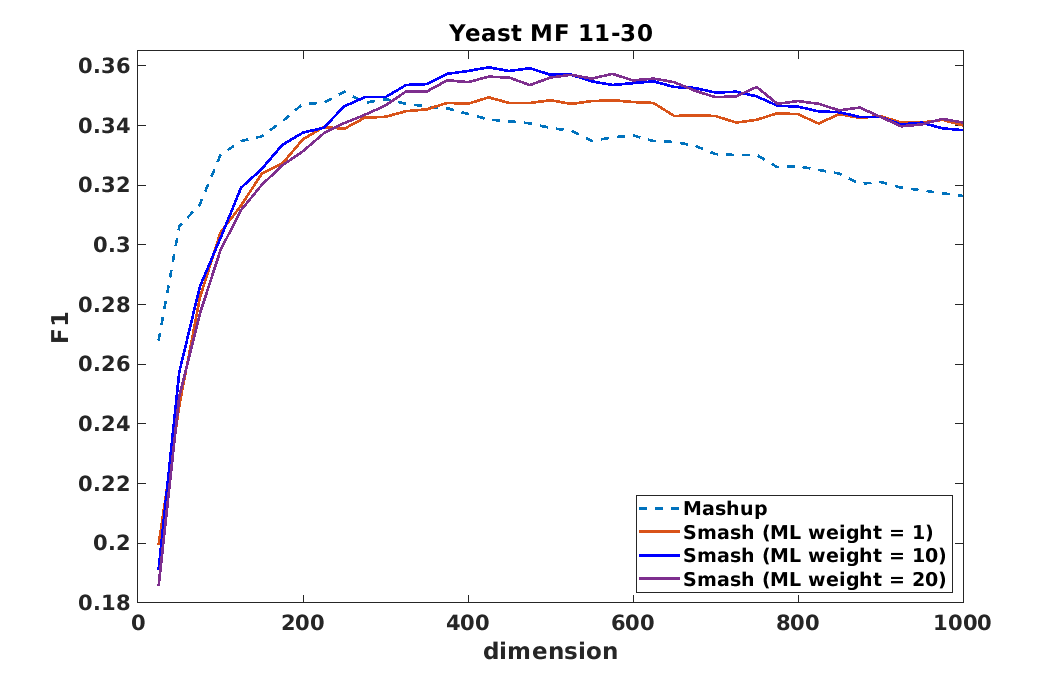
\includegraphics[width=.8\linewidth]{Yeast-MF-11-30-F1}  \\
	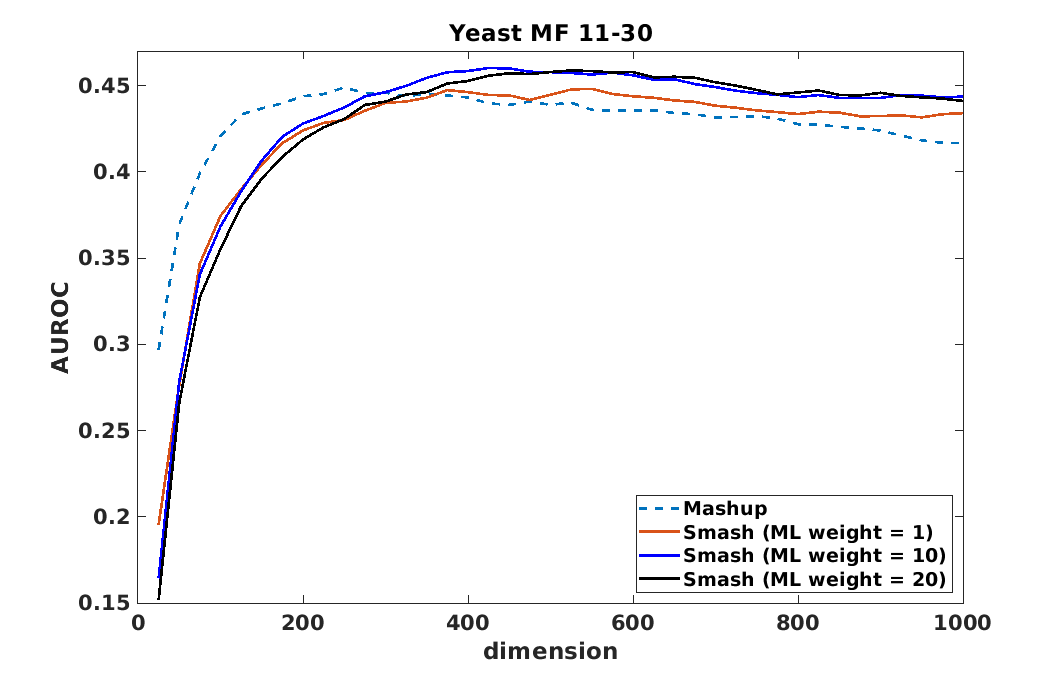
\includegraphics[width=.8\linewidth]{Yeast-MF-11-30-AUROC} 
	%\caption{Yeast BP}
	%\label{fig:yeast-bp}
\end{figure}

\begin{figure}[h!]
	\centering
	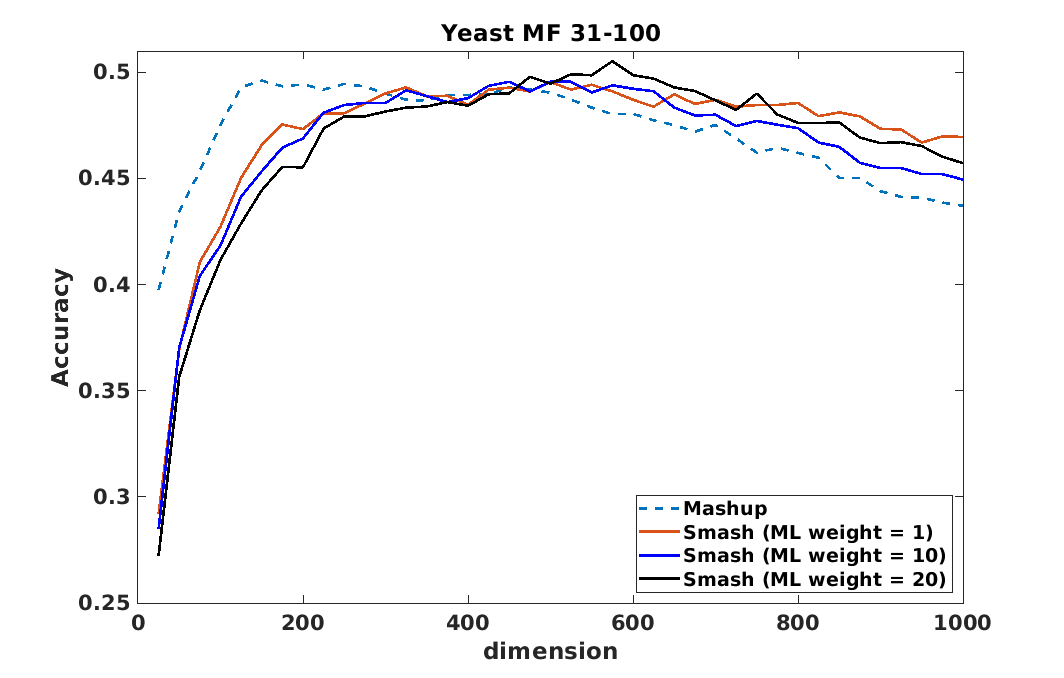
\includegraphics[width=.8\linewidth]{Yeast-MF-31-100-Acc}  \\
	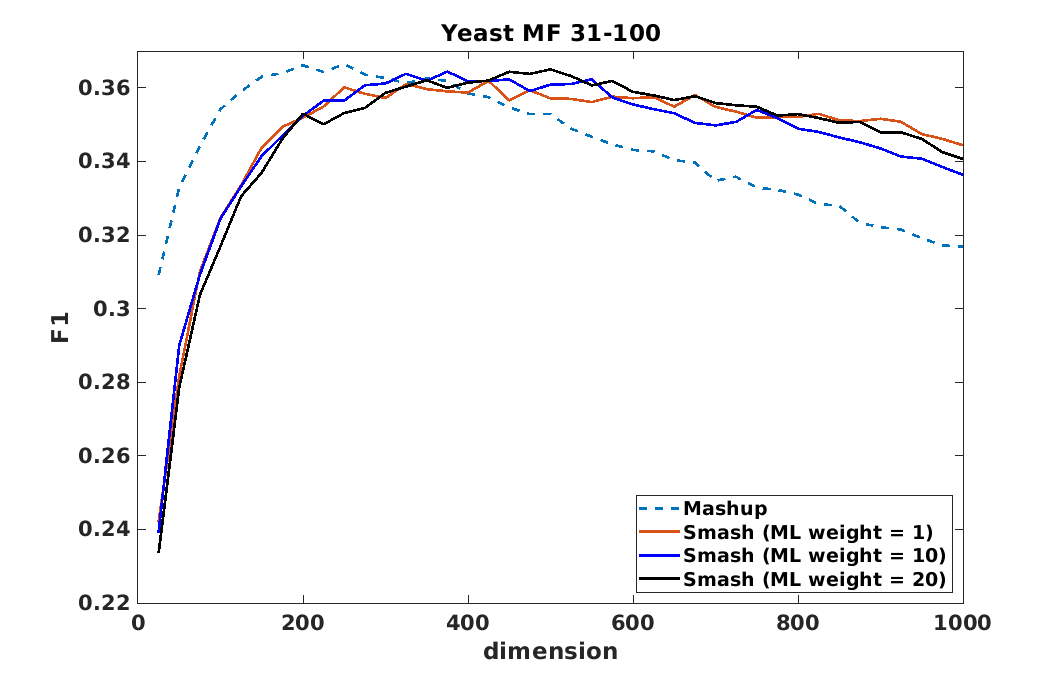
\includegraphics[width=.8\linewidth]{Yeast-MF-31-100-F1}  \\
	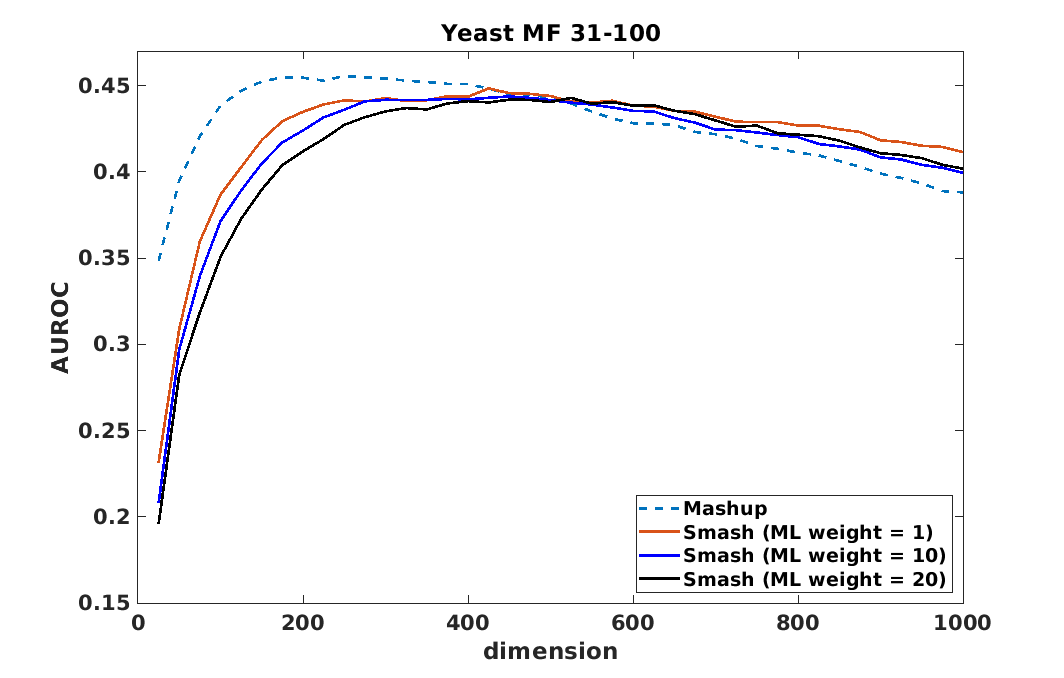
\includegraphics[width=.8\linewidth]{Yeast-MF-31-100-AUROC} 
	%\caption{Yeast BP}
	%\label{fig:yeast-bp}
\end{figure}

\begin{figure}[h!]
	\centering
	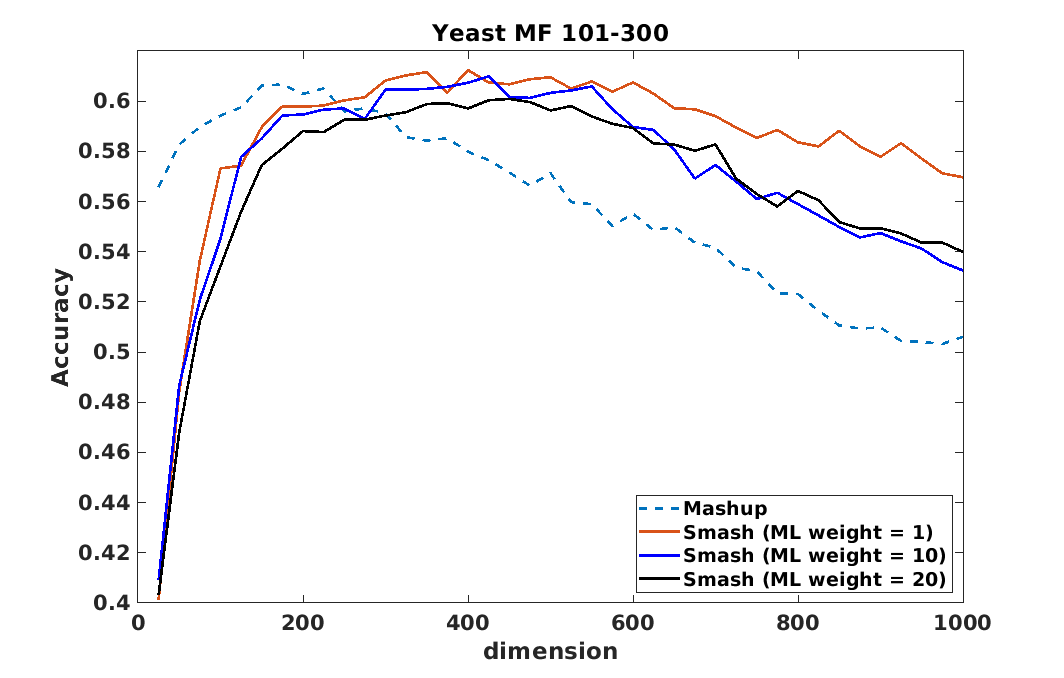
\includegraphics[width=.8\linewidth]{Yeast-MF-101-300-Acc}  \\
	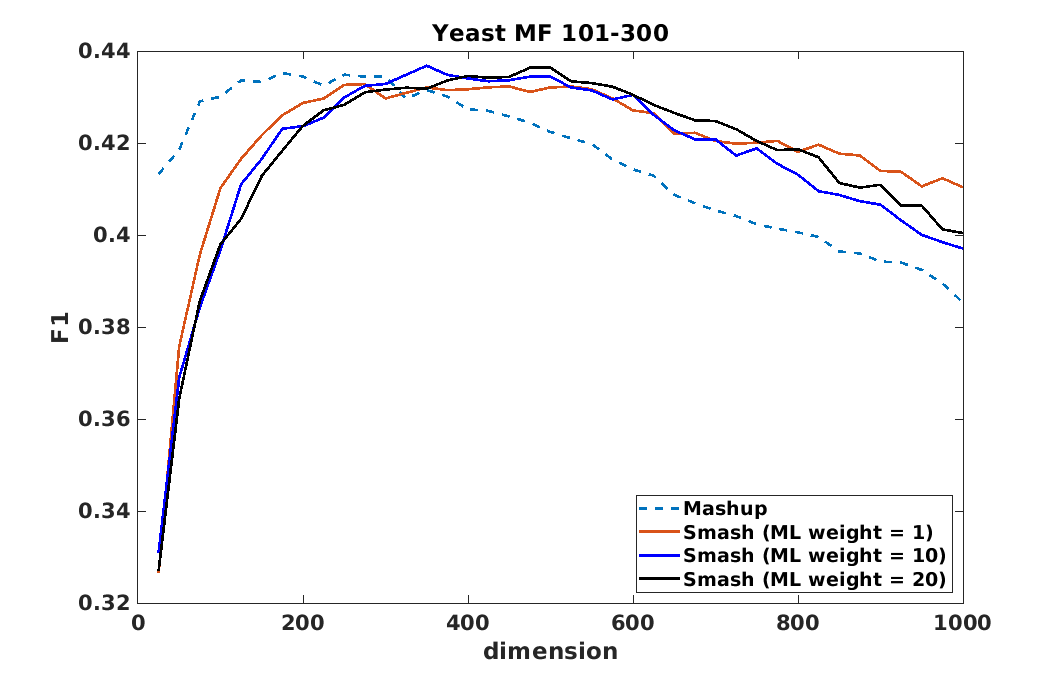
\includegraphics[width=.8\linewidth]{Yeast-MF-101-300-F1}  \\
	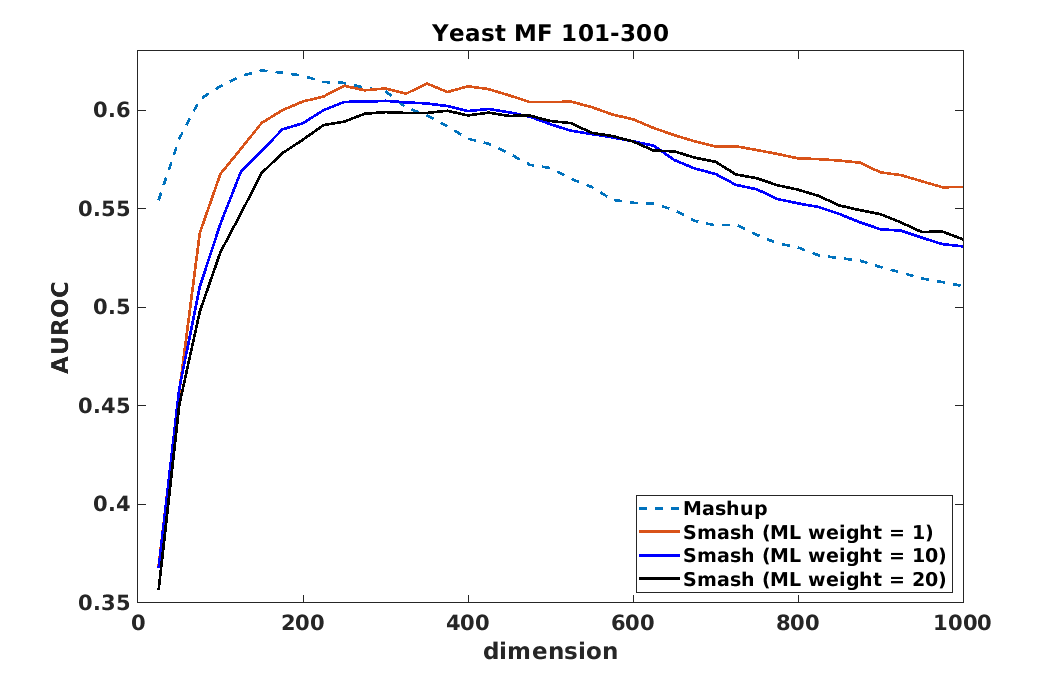
\includegraphics[width=.8\linewidth]{Yeast-MF-101-300-AUROC} 
	%\caption{Yeast BP}
	%\label{fig:yeast-bp}
\end{figure}

\end{document}  